\documentclass[../main.tex]{subfiles}
% 1.1 Spektroskopie
% 1.1.1 Was ist es generell?
Spektroskopie ist ein Überbegriff für analytische Verfahren, die elektromagnetische Strahlungen zerlegen. Die gemessene Strahlungsintensität im IR-Spektralbereich liefert ausschlaggebende Information über die molekulare Zusammensetzung einer Substanz.

% 1.1.2 Was ist Prisma-Spektroskop?
Als Beispiel zerlegt ein Prismenspektrometer sichtbare Strahlung mit einem Prisma. Das resultierende Spektrum offenbart bei Sonnenlicht alle Wellenlängen bzw. Farben im sichtbaren Wellenlängenbereich (ca. 400nm-700nm) \cite{TODO}. Auch zu erkennen sind dunkle Linien bei bestimmten Wellenlängen (Abb. \ref{fig:fraunhofer-linien}). Diese werden als Absorptionslinien oder \textbf{Fraunhofer'sche Linien} bezeichnet.

\begin{figure}[ht]
    \centering
    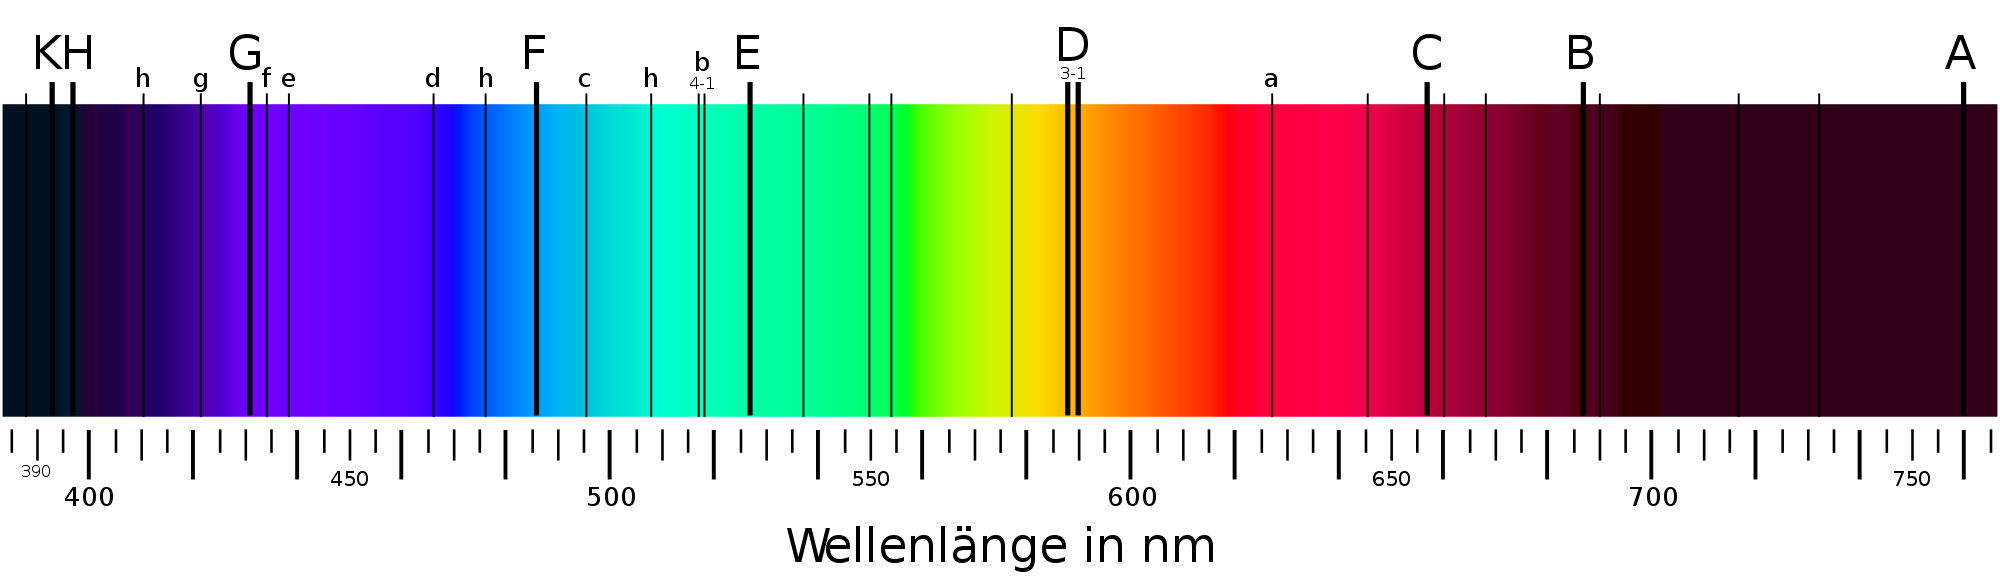
\includegraphics[width=0.65\textwidth]{fraunhofer_linien.png}
    \caption{Fraunhofer'sche Linien im Sonnenlichtspektrum \cite{fig:fraunhoferlinien}}
    \label{fig:fraunhofer-linien}
\end{figure}

% 1.2 Fraunhoferlinien
% 1.2.1 Entdeckung Fraunhofer
Joseph Fraunhofer entdeckte und dokumentierte 1814 sorgfältig über 570 dieser Linien \cite{fraunhofer_entdeckung}. Mit seinen Ergebnissen konnte er hochwertige astronomische Fernrohre herstellen.

% 1.2.2 Entdeckung Bunsen, Kirchhoff
1859 führten Gustav Robert Kirchhoff und Robert Bunsen ein Experiment durch, bei dem eine Assoziazion zwischen chemischen Elementen und den Fraunhofer'schen Linien beobachtet wurde \cite{TODO}. Daraus folgt, dass die Absorptionslinien des Sonnenspektrums, welche Fraunhofer analysierte, die Absorptionseigenschaften dieser Elemente reflektieren.

% 1.3 IR-Spektroskopie
% 1.3.1 Was ist es?
Die IR-Spektroskopie ist eine Methode der Molekülspektroskopie, welche sich mit den zwischenmolekularen Kräften in Molekülstrukturen beschäftigt. Bei der Infrarotspektroskopie werden Wellen im Infrarotbereich (ca. 800nm-1mm) \cite{TODO} zerlegt.

% 1.3.2 Vgl. Fraunhofer
Genau wie bei Fraunhofers Lichtspektrometer dient die Infrarotspektroskopie dem Nachweis chemischer Stoffe. Während das Lichtspektrometer die chemische Zusammensetzung der Sterne durch die Absorption am sichtbaren Licht der dortigen Elemente nachweist, kann das Infrarotlicht eines IR-Spektrometers Schwingungen in bestimmten chemischen Gruppen anregen \cite{TODO}, und somit in gewissen Wellenlängenbereichen Absorptionen herbeirufen.

% 1.3.3 Methoden: FTIR, Laser, Raman, ATR, etc.
Zu den Arten der IR-Spektroskopie gehören u. A. FTIR-, Raman-, und ATR-Spektroskopie.
